\documentclass{article}

% luc specific commands

\newcommand{\code}[1]{\texttt{#1}}
\newcommand{\codeblock}[1]{\vspace{1mm}\noindent\begin{center}\texttt{#1}\end{center}\vspace{1mm}}
\newcommand{\coati}{\textsc{Coati}\xspace}
\newcommand{\grph}{\textsc	{Grph}\xspace}
\newcommand{\jalinopt}{\textsl{\underline{J}a\underline{l}in\underline{o}pt}\xspace}
\newcommand\toools{\texttt{T\textbf{ooo}ls}}



\usepackage{xspace}
%\usepackage[colorlinks,linkcolor=black]{hyperref}
\usepackage{url}
\usepackage{listings}
\usepackage{color}





\definecolor{ornge}{RGB}{230,230,230}
\lstset{
basicstyle=\footnotesize, 
backgroundcolor=\color{ornge}, 
numbers=left
}


\setcounter{tocdepth}{2}


\title{\grph: an efficient portable graph library tailored to network simulation
and graph analysis}

\usepackage{pdfpages}

\begin{document}

\maketitle
\begin{footnotesize}
\vfill
\tableofcontents
\end{footnotesize}
\newpage

\begin{abstract}
\end{abstract}

\section{Introduction}


\subsection{General description}


Many scientific and technical fields relate to graphs. Researchers and
engineers who need to programmatically manipulate graph structures have access  to a number of existing graph frameworks \cite{jungweb, 504206, jgraphtweb, sageweb}. 
Unfortunately, in spite of the intrinsic qualities of each specific framework, their all turn out to have strong limitations
in either their execution platform, their computational performance,  the
flexibility of their graph model, etc.
As a consequence scientists most often opt for developing 
ad hoc  tools. The very same code is then invariably re-written by different groups of people, providing 
the same functionality and exhibiting the same mistakes. These mistakes include inappropriate design and implementation techniques which lead to poor performance and thereby the unability to deal with large graphs.

\grph is a Java graph toolkit enabling experimentation on large graphs (in the order of millions  nodes).
It proposes a general graph models which supports
directed and undirected simple and hyper-edges in a mixed fashion. Its design and implementation objectives are geared towards:
\begin{itemize}
  \item computational efficiency;
  \item memory efficiency;
  \item simplicity.
\end{itemize}

To this purpose, \grph exhibits  the following features:
\begin{itemize}
  \item a data model which represents vertices and edges as positive integers;
  \item a efficient data structure based on incidence lists;
  \item implementations for most common graph algorithms;
  \item a framework for the development of new algorithms and their integration with \grph;
  \item a graphical monitoring interface;
  \item a console-based interactive interface (shell).
\end{itemize}


\subsection{State of the Art}
Several graph frameworks are available to the graph community. Most relevant
frameworks include
Mascopt \cite{LSV04}, GraphStream \cite{Dutot2007}, Boost \cite{504206}, LEDA,
JGraphT \cite{jgraphtweb}, JUNG \cite{jungweb}, SAGEMath \cite{sageweb}, etc.

This document focuses on Java software, hence it does not  consider greats tools like Boost or LEDA, which are in C++
or SAGEMath which is implemented in a mix of Python and dialect of C, called Cython.

Java users can choose in a plethora of frameworks. Most of them are lab tools which still are at an early stage of their development and would not
be used in a production environment. Mature graph projects include JUNG, Apache Maths Commons and GraphT stand among the most often used.
Unfortunately most of these frameworks suffer from a lack of
support for certain class of graphs (mixed graphs, hypergraphs), from an often complex design, and from poor performance.
In particular their full-OO design (which allows the construction \code{Graph<V, E>} when V and E can be
of any type) imposes their implementation to rely on hashtables. The immediate consequence of using hashtables in Java
is the large memory usage and slow access time (even is hashtables  theoretically operate in constant time, they prove
 much slower than arrays).  

\subsection{Motivation}
Our initial motivation for the \grph project was to build up a graph toolkit that would help us in the frame of
a Research project at Inria labs, whose the problem was the simulation of large networks. Later we realized the potential
of our graph toolkit to compete with the best ones. 
Then our motivation changed: our aim is now to deliver that can help anyone researcher or engineers in need of graph-related
functionality, wether it be in academical research of industrial context.

\subsection{Why calling it \grph?}
Why have chosen \grph as the library name. The toolkit was initially called \textit{Dipergrafs} (at the time it was related to Inria project) because it focused on
the manipulation of directed hypergraphs. Since the objectives have somehow changed, the name had to be adapted.
Now the target model is general graphs mixed in terms of the nature of the edges (simple and hyper) and in their
directivity (directed or not). We opted for ``Grph'' because the missing 'a' retains lots of attention and  it is short enough
so it can be used within the API.


\section{Quick start}

The objective of this section is to briefly give the user the hints on how to
use \grph.



	The  parameters of \grph methods are always checked. To
	this purpose, and for the sake of performance, \grph uses assertions. 
	
	Unfortunataly, the JVM disables assertions by default. They can be enabled in two ways:
	
	\begin{itemize}
  \item by using the \code{-ea} flags on the JVM command line;
  \item or by executing the following line of code before any reference to the
  \code{Grph} class.
		\codeblock{ClassLoader.getSystemClassLoader().setDefaultAssertionStatus(true)}
\end{itemize}


\subsection{Creating a graph}

To create an empty graph, just do:

\codeblock{Grph g = new InMemoryGrph();}


\subsubsection{Adding vertices and edges}

Adds a new vertex (using the lowest ID available):

\codeblock{g.addVertex();}


Adds a given vertex:

\codeblock{g.addVertex(v);}



\subsection{Common topologies}

The utility class \codeblock{ClassicalGraphs} provides a set of methods for the generation of classical
graph topologies like grids, paths, cycles, peterson graphs, etc.


\subsection{Displaying a graph}

The default \codeblock{display()} methods displays the graph. The stategy employed to display is chosen by the library, since it depends on the type of the graph. It may also vary upon the different version of Grph.

Until now, the display relied on the GraphStream library. In the future, GraphStream will be replaced by
a faster and lighter graph drawing toolkit.


\section{Models}

\subsection{Graph model}
Historically, the initial motivation for developing \grph was to make it useful in the context of network simulation,
considering that networks involve a number of different technologies that must be modeled in their own
special manner: Ethernet bus, optical links, Wi-Fi/Bluetooth wireless networks, duxplex/full duplex communication channels, etc. 
Undirected/directed simple/hyper edges provide the adequate abstractions to represent this technological variety.


Then  \grph comes with a general graph model that supports:
\begin{itemize}
  \item simple graphs;
  \item multigraphs;
  \item hypergraphs;
  \item any undirected, directed or mixed versions of these (mixed graphs);
\end{itemize}


\subsection{Vertices and edges model: the use of the int primitive type}
Most graph toolkits provide models for graphs of \textit{objects}: they allow vertices and objects to  be of any type. This elegant OO design
has a rude counterpart: it prevents good performance because it requires:
\begin{itemize}
  \item the computation of hashcodes;
  \item the use of hashtables, which have heavy memory footprint, and exhibit slow operation;
  \item the use of pointers, which require 64 bits on modern computers and add indirections;
  \item the user of objects, which have large (at least 12 bytes) overhead.
\end{itemize}

\grph follows another approach, geared toward  performance:
it models vertices and edges as numbers. These number are stored in contiguous sequences of native integer values, which
removes the need to hashcode, hashtables, pointers and objects.

The spaces of identifiers do not have to be contiguous, though the data structure exhibits the best
memory performance when these spaces are dense.

\subsection{Properties}


\grph define a number of basic properties for vertices and edges:
\begin{description}
  \item label (one String object);
  \item color (4 bits);
  \item edge-width (4 bits)  and vertex-size (4 bits);
  \item edge-style (1 bit) and vertex-shape (1 bit)
\end{description}

These properties all have an obvious graphical representation, and are actually used in the monitoring view and
Graphviz/DOT export method. 

The user can replace these properties by define its own property objects.



\subsubsection{Searching properties}

\textit{Note: the mechanism of index is disabled in 2014 version of Grph. It may be re-introduced later on.}

The property framework \grph features a function which returns a set of elements that have a given value for a given property.
This method is \codeblock{IDSet IntProperty.findElements(int value)}

This function iterates on the set of elements by storing elements that are found to have the requested value.
If the performance of this search function is critical to your application, you may want to index
the value of properties for set of elements that store it. This strategy is commonly used in database systems where is it referred to as \textit{cursor}.
A property can be asked to use a cursor via its \code{setUseCursor(boolean)} method.  
The complexity of the search operation is then:
\begin{itemize}
  \item $\Theta(1)$ if the cursor is used;
  \item $\Theta(n)$ otherwise.
\end{itemize}

Using a cursor improves the search of elements when the number of element is large but it significantly slows down the operations:
\begin{itemize}
  \item changing the property value for elements;
  \item adding/removing elements from the graph.
\end{itemize}

\subsubsection{Managing graphs of objects}
Although this model matches well the mathematical concept of a graph and is adequate to developments that come atop \grph, 
many situation still require the vertices and/or edges to be modelled as objects (for the example when the data model was
defined prior to the decision of using \grph).

\grph solves this issue by providing a bridge from the object world to the integer world, and the other way around.
The class \code{grph.oo.ObjectGrph<V, E>} encapsulates an instance of an integer-based graph and provide
the necessary conversion methods: from IDs to objects (vertices or edges) and from set of IDs to sets of objects.

Because of the number of API methods \grph available to the developer is large, the class \code{ObjectGrph<V, E>} cannot
reasonably bridge all of them. \grph considers that the conversion methods provided will serve the user at implementing the  
object-based methods he needs, by bridging the already  integer-based methods available.


\section{Data structure}

\grph comes with one single implementation for the graph data structure which is based on four coupled incidence lists.
It is commonly admitted that incidence list based implementation perform well when graphs are sparse and that dense graphs
are more adequately represented by matrices. In practice, people dealing with dense graphs are theory animals who
seldom opt for programmatic solutions anyway.

The incidence lists used by \grph store the IDs of incident elements. They are indexed by the ID of element they relate to.
The cell at index $n$ in the vertex incidence list contains the set of ID of the edges incident to vertex $n$. This
cell is left empty if vertex $n$ is not in the graph.

\subsection{Element sets}

Many functions returns set of ID (either vertex IDs or edge IDs). For the sake of performance \grph may return references to
ID sets that are used internally, instead of returning copies. Altering the content for these set would compromise
the integrity of graphs. To this purpose, the returned sets are flagged, indicated weather they are internal sets.


 \subsection{Property value}
 
 The way the basic property values are stored is up to the developer. Within \grph, default properties are stored in dedicated arrays
 which allow small memory usage.
 
 In order to capture the benefit of using this strategy, consider as an example a \textit{marked} vertex property that can take two values.
 The smallest data types in Java that can be used to store a rank value are boolean or bytes (both are encoded on 8 bits).
\begin{itemize}
  \item if vertices were modelled as objects, every vertex would occupy 192 bits of memory: 12 bytes of Java object overhead) + 1 byte
  for the mark (but actual size of the object would be 16 bytes because the size for any java object must be multiple of 8) + 64-bit reference to the vertex;
  \item in the case vertices are modelled as numbers,
the space required to store one vertex and its \textit{marked}  is 33 bits: 32 bit integer for the vertex ID + 1 bit for the boolean value
(that can be stored in a bitset storing all \textit{marked} values for all vertices).
\end{itemize}
This example, which represents a very common situation, shows a memory usage that is 5.8 times lower when using integer vertices. 
 
 
 
\subsection{Computational complexity}
This model exhibit the following computational complexity:

\begin{description}
  \item[number of elements] is the number of non-empty cells in the list; since the number of empty cells is stored and
  updated on-the-fly, computing the number of elements simply consists in substracting the number of empty cells to the
  actual size of the incidence list; this is done in all case $0(1)$;
  \item[looking up an element] is done by checking if a cell a the given index is empty or not; this is done in $0(1)$
	\item[adding an element] is done by setting a cell at the index given by the ID of the the element with an instance of an object storing the IDs of its incident elements; this is done in $0(1)$;
  \item[removing an element] is done by emptying a cell at a given index and updating the incident set of its incident elements; this
  is done in $0(n)$, $n$ being the number of elements incident to the  element to be removed --- its degree;
  \item[iterating over the elements in the set] is done by sequentially iterating over the list, ignoring empty cells; this is done
  in $0(n + m)$, $n$ being the number of elements of the corresponding type in the graph and $m$ the number of empty cells in
  adjacency list. Most often $m$ tends to zero.
\end{description} 

Compared performance shows that using HPPC for manipulation vertices/edges is 7 time faster than using Java collections when
it comes to creating them, and 2.5 times faster when it comes to iterating over them.



\subsection{Memory complexity}

The incidence of every element (vertex or edge) is represented by an object.
\begin{itemize}
  \item a simple edge, either directed or not, takes 20 bytes: 4 (ID)+16 (incident vertices)
\item  an undirected hyperedge takes $4+16+12+n\times 4$, $n$ being the number of incident vertices.  
\item  a directed hyperedge takes $4+24+n\times 4$, $n$ being the number of incident vertices.  
\item a vertex takes 4+24 bytes.
	\begin{itemize}
	\item adds $12 + n\times 4$ if it has $n$ out directed edges;  
	\item adds $12 + n\times 4$ if it has $n$ in directed edges;  
	\item adds $12 + n\times 4$ if it has $n$ undirected edges;  
	\end{itemize}
\end{itemize}

A graph with $n$ vertices and $m$ edges takes $24 + n(40+4\frac{m}{n}) + 20m$ bytes.


\section{Algorithms}

\grph comes with implementations for most common graph algorithms as well as with a framework for the implementation and integration
of new ones.

A convention within \grph is that all algorithms are usable through public
methods in the \code{Grph} class. These methods can be straight implementations of algorithms or, better, facility method that
call {\em algorithm objects}.
This design may be subject to criticism because it leads to a cumbersome \code{Grph} class. On the other side, Integrated Development
Environments (IDEs) such as Eclipse or Netbeans come with code-completion
functionality that all users intuitively use and that make navigation in large source codes easy.









\section{Quest to the maximum performance}

\grph makes use of a number if strategies to improve it overall performance. This strategies are detailed in this section. 

\subsubsection{Caching}

In order to improve even more the computational efficiency for the previously mentioned algorithms,
\grph makes use of a {\em cache}.
	  \begin{itemize}

\item Basically, any given property will not be computed twice if the graph has not changed since then.
This {\em improves} the complexity of graph operations.
\item For example, the computation of all-pair shortest paths will return immediately if 
the diameter  was previously computed . This is because both algorithms rely on a
BFS that was first computed by the ``diameter algorithm''.	
	  \end{itemize}
	  Depending on the application, performance  may dramatically improves.

Practical experiments show that most time is wasted by computing several times the same
algorithms on the same graphs, either directly or not.

In order to avoid this, \grph provides a built-in mechanism which stores the
results of calculations until a change occur in the structure of the graph. Changes include
vertex or edge removal or addition. By default, property changes on vertices or edges are not
taken into account (because \grph has no mean of detecting them).

Consequently, between two changes of the graph structure (it is also likely that the graph
is static, e.g. is will never change), the first invocation of a given graph operation
will be performed in the theoretical time complexity, while each subsequent one will be
performed in constant time --- it actually won't be performed at all, since the cache will bypass it.

When a change occurs (event the slightest
one), the entire cache is cleared. 


If you want you algorithm to take benefit of the caching mechanism, you simply need to wrap it
into a \code{CachingGraphAlgorithm}  object. The following code does it for you:
\begin{lstlisting}
class MyGrph extends Grph
{
	private MyAlgo myAlgo = new MyAlgo().cache(this);
	
	public int getMyValue()
	{
		return myAlgo.compute(this);
	}
}
	
\end{lstlisting}By doing this, the result provided by your algorithm will be cached until a topological change occur in the graph.
The benefit of the caching mechanism is higher when the graph is little dynamic and when computations and time-consuming.


\subsubsection{On-demand processing}

Processing is done only when the result is requested. This avoids useless processing.


\subsubsection{Using native code}

Most critical algorithms are implemented in C and compiled to the target machine.
These algorithms are called {\em native algorithms}. Like all algorithms in \grph, a native algorithm
comes in the form of a Java class. A native algorithm additionally  come with a C file. When the algorithm 
is first executed, \grph compiles the C source by using optimizations for the local machine. To do this, the
gcc compiler must be available on the corresponding computer. If the C code cannot be compiled, an optional
alternative 100\% pure Java algorithm is executed.

Many people complain about the poor performance of Java implementations. Our experiments show that
 C implementations are about 5 times faster than equivalent Java ones.

\grph provides a framework for the development of C implementations for graph algorithms.
In order to use it, you need to write the C implementation in the form a set of C functions.
Then you need to write a Java interface declaring these C functions, in a way similar to C header files.
Then you need to extends the \code{AbstractNativeGraphAlgorithm} class in order to provide
the translation of data between Java and C. At runtime, the C implementation will be compiled
on the fly using the local C compiler. The resulting native code will be dynamically loaded and executed.

To write the C code, 
create a new file called \code{MyNativeAlgorithm.c}, aside to your java source file:

\begin{lstlisting}
interface MyNativeAlgorithmNativeInterface extends Library
{
	int computeSum(int n, int* vertices)
	{
		// C code...
	}
}
\end{lstlisting}


You need to declare the native function that will be loaded, as shown in the example:

\begin{lstlisting}
interface MyNativeAlgorithmNativeInterface extends Library
{
	int computeSum(int n, int[] vertices);
}
\end{lstlisting}

To call the C functions from Java,  you need to declare the algorithm class:

\begin{lstlisting}
public class MyNativeAlgorithm extends AbstractNativeGraphAlgorithm<Integer, NativeAlgorithmFunctions>
{
	@Override
	protected Integer nativeCaller(Grph g)
	{
		((MyNativeAlgorithmNativeInterface) getNativeInterface()).computeSum(list.length, list);
	}

	@Override
	protected Class<NativeAlgorithmFunctions> getNativeFunctionsDescriptor()
	{
		return MyNativeAlgorithmNativeInterface;
	}

	@Override
	public String getName()
	{
		return "test native";
	}

	@Override
	public String getDescription()
	{
		return "test native";
	}
}
\end{lstlisting}


If the native source code is other than C, then you need to specify how to compile it. For example,
the use of C is defined by the single following line:

\begin{lstlisting}
AbstractNativeGraphAlgorithm.compilers.put("c", "gcc  -O3 -o $LIB -shared -static -lc $SRC");
\end{lstlisting}

The \code{\$LIB} and \code{\$SRC} variable will be replaced by the name of the source file and library file that the
compiler will generate.

Better avoid native algorithms.




\subsubsection{Data wrapping}

In order to avoid the construction new large data structure based on other ones, \grph makes an extensive use
of wrappers. Wrappers are objects that store nothing but simply redirect call to other data structures.

For example, shortest paths do not store a sequence of vertices. They have a reference to the distance and 
predecessor matrices that provide the necessary information for the shortest paths. This mechanism makes a shortest path of length
10 weigths 4 bytes instead of 56 bytes, hence 14 times shorter.




\subsubsection{Parallelism}

Modern computers embed a multi-core processor, enabling threads and processes to run
in parallel. In order to take advantage of this parallelism,
whenever possible \grph split the computation in a number of independant jobs that are executed 
in parallel, within distinct threads,  on the local computer.

Depending on the algorithms, the speed off varies from near-to-zero to $n$,$n$ being the number of processors/cores available on the computer. 

\grph comes with a basic parallelization framework for the execution of a certain class of algorithms: if an algorithm can be decomposed
in   routines called independently on every vertex, it may be invoked by the following code pattern:



\subsubsection{Disabling assertions}	
		
The code of \grph makes an extensive use to assertions. This tends to improve the quality of the source code.
Contrarily to the recommandations, \grph uses assertions for method parameters checkings too.

This enables the user to disable the assertions, hence disabling all verifications, making the execution significantly faster.

The disadvantage is that the user must not forget to include the following line before the first call
the the \code{Grph} class, in order to enable error verification during the development process.

		\codeblock{ClassLoader.getSystemClassLoader().setDefaultAssertionStatus(true)}
		


\subsubsection{Profiling algorithm implementations}

Many researchers in algorithmics are interested in performance issues. In order to facilitate the study of the performance for
algorithms, \grph provides a set of methods enabling to know the duration spent computing. 

The implementations of the algorithms that \grph uses are the ones that suits better its data structure.

		

\section{Advices for writing fast code}

\subsection{Iterating}

Instead of iterating using \code{IntCursor}, like it is done in HPPC:
\begin{lstlisting}
for (IntCursor c : set)
{
	int e = c.value;
}
\end{lstlisting}
It is generally faster (although more eager of memory) to first convert the set to an array and iterate over the array, like this:
\begin{lstlisting}
for (int e : set.toIntArray())
{
}
\end{lstlisting}
If the set does not change, this method is dramatically faster. If the set does change all the time, this method is a little slower.




\section{Graph import/export formats}

	\grph provides a set of bridges which make it interoperable 
	with a number of external tools. This interoperability enables persistence,
	dynamics, two-dimensional rendering (both static
	and dynamic), etc. The coming sections detail the interoperability
	capacities of \grph.



\subsection{\grph native formats}

\grph natively defines two graph import/export formats: GrphBinary and GrphText. 

\subsubsection{GrphText: the text \grph Language}

GrphText is an extension to the common adjacency list  format used by Inet, CAIDA maps, etc.
It extends it by offering the ability to describe:
\begin{itemize}
  \item directed edges;
  \item directed and undirected hyper-edges (bus);
  \item half and loose edges (edge with one or no end);
  \item edge identifiers.
\end{itemize}

GrphText imposes that vertex and edge identifiers are positive integers.
The directivity of an edge is described by the use of the character $>$.
Edge identifiers are optional: if they are not given, \grph will assign them itself
using the natural order $0 1, 2, 3, etc$.

The format for an ID, called $id$ is then \code{[0-9]+}. The format for an edge declaration is
then: \codeblock{(id:)? id* >? id*}.

As illustrated in the following examples, the compact syntax of GrphText enables the representation of any graph topology.



\begin{center}
\begin{tabular}{|l|r|}
\hline
\textit{The line} & \textit{Describes\ldots} \\
\hline
\code{1 2} & an undirected edge connecting vertices 1 and 2 \\ 
\code{2 > 3} & a directed edge from 2 to 3 \\ 
\code{1: 2 > 3} & the same, but the edge ID is set to 1 \\ 
\code{8} & an isolated vertex with ID 8 \\
\code{\{8\}} & an undirected hyper-edge that contains vertex 8 \\
\code{2: \{8\}} & an undirected hyper-edge of ID 2, and that contains vertex 8 \\
\code{\{8 4 5 7\}} & an hyper-edge connecting vertices 8, 4, 5 and 7 \\
\code{\{8 4\} > \{5 7\}} & a directed hyper-edge connecting vertices 8, 4 to 5 and 7 \\
\code{\# a comment} & guess what\ldots \\
\hline
\end{tabular}
\end{center}

In GrphText, blank lines are ignored. If a \code{\#} is found, it is assumed that the
rest of the line is a comment.


\subsubsection{GrphBinary:  the binary \grph Format}

GrphBinary provides a compact encoding for graphs.  

The number of bytes used for the storage of IDs is computed from the total number of elements.
If less than $2^8$ elements have to be stored, they one byte will be used to store the IDs.
If less than $2^16$ elements have to be stored, they two bytes will be used to store the IDs.
Otherwise 4 bytes are used.

The GrphBinary format is based on the encoding defined by \code{java.io.DataOutputStream} and is organized  as follows:
\begin{enumerate}
  \item the name of the graph class;
  \item whether the vertex/edge properties will be written in the file or not
  \item whether the cached values for algorithms will be written in the file or not
  \item the topology, which is decomposed as follows:
  \begin{enumerate}
    \item the greatest vertex and edge IDs;
    \item the number of isolated vertices, following by all of them;
    \item the number of undirected simple edges, then for each of them:
	  	\begin{enumerate}
	  	\item its number;
	  	\item its two adjacent vertices.
		\end{enumerate}
    \item the number of directed simple edges, then for each of them:
	  	\begin{enumerate}
	  	\item its number;
	  	\item its source then its destination.
		\end{enumerate}
    \item the number of undirected hyper edges, then for each of them:
	  	\begin{enumerate}
	  	\item its number;
	  	\item the number of incident vertices followed by all of them.
		\end{enumerate}
    \item the number of directed hyper edges, then for each of them:
	  	\begin{enumerate}
	  	\item its number;
	  	\item the number of tail vertices followed by all of them.
	  	\item the number of head vertices followed by all of them.
		\end{enumerate}
    \end{enumerate}
  \item the number of graph properties then, for all of them:
  	  	\begin{enumerate}
	  	\item its name;
	  	\item its property-dependant binary encoding;
		\end{enumerate}
  \item the number of graph algorithms that use caching then, for all of them:
  	  	\begin{enumerate}
	  	\item its name;
	  	\item the Java serialization binary encoding for the cached value.
		\end{enumerate}
\end{enumerate}


\subsection{Others}

\subsubsection{Dimacs}

\subsubsection{LAD}


\subsubsection{DGS}
	
		DGS (Dynamic Graph Stream) propose a  language for the description
		of dynamics in simple graphs, directed or not.
		Practically a DGS stream (coming from a file, a URL, etc) defines
		a sequence of steps in which a number of events occur. Possible
		events include: creation/deletion of a node, creation/deletion of
		a link, modification of the value for a node/link attribute.
		
		\grph provides DGS drivers which
		make it possible to:
		\begin{itemize}
			\item animate a graph using the DGS language;
			\item generate DGS text out of the events which happen
			on the graph (e.g. manipulating a graph though its API entails
			the generation of the corresponding DGS instructions). 
		\end{itemize}

\subsubsection{GraphViz dot}
		Graph visualization is a way of representing structural information as
		diagrams of abstract graphs and networks. Automatic graph drawing has many
		important applications in software engineering, database and web design,
		networking, and in visual interfaces for many other domains. 
	
		Graphviz is open source graph visualization software. It takes as input
		a description of a digraph and is able to ouput a variety of popular
		graphic formats (both bitmap and vector-based). 
	
		\grph comes with a GraphViz driver which allow the user to 
		export the graph as GraphViz text. In the case of dynamic graphs,
		only snapshots can be generated since GraphViz does not consider
		dynamics. In this case GraphStream can be used.
	
	\subsubsection{DotML}
	Under progress
		
\subsubsection{GraphML}
\begin{lstlisting}
<?xml version="1.0" encoding="UTF-8"?>
<graphml xmlns="http://graphml.graphdrawing.org/xmlns">
	<graph id="1220081709" edgedefault="directed">
		<node id="100" />
		<node id="98" />
		<node id="99" />
		<node id="97" />
		<edge source="97" destination="98" />
		<edge source="97" destination="99" />
		<edge source="98" destination="100" />
	</graph>
</graphml>
\end{lstlisting}

\subsubsection{GML}
\url{http://www.infosun.fmi.uni-passau.de/Graphlet/GML/}


\subsection{Sharing instances}
If you wish to share an instance of a given graph, you can store it to a file on disk and send this file via e-mail.
Another solution consists in uploading the graph using the \code{Grph.post()} method. This method will return an URL
that you must give to the people you want to send the graph to. These users will be able to load the instance via the 
\code{Grph.loadOnlineGrph(url)} method.


\subsection{Monitoring}

For monitoring purpose,
it relies on the simple yet powerful Graphstream.

		GraphStream is an open source  library which allows
		the two-dimensional rendering of dynamic graphs.
		GraphStream listens to graph changes
		(node/edge creation/deletion and node/edge attribute value modification)
		and automatically updates the graphical representation. It uses
		an algorithm providing automatic balancing.
		
		
		
		

		
\section{Installation}

If you plan to use \grph through its API, then you need to download the JAR files on \grph website and add them to your CLASSPATH.

If you plan to use the experimentation console then you need to install \grph on your computer by issueing the following command at your
shell promt:
\codeblock{curl -s http://www-sop.inria.fr/members/Luc.Hogie/java4unix/j4uni | sh -s grph }

This command downloads the last version of \grph and install it in the \code{\$HOME/.grph} directory.
The commands will be copied to the directory \code{\$HOME/.grph/bin} and the jar files will be in
\code{\$HOME/.grph/lib}.

\section{Third-party software}
In order to achieve these goals, it relies on the following third-party software:
\begin{description}
  \item[GraphStream] is a dynamic graph visualization toolkit. 
  \item[HPPC] is a framework for efficient manipulation of Java primitive types.
  \item[BeanShell]
   \item[Java4unix] 
  \item[JLine] 
\end{description}


\section{User interaction}

\subsection{Reporting}

\begin{lstlisting}
~$ grph-console 
	Grph g = new InMemoryGrph();
	g.createVertices(30);
	g.glp();

	Report report = new Report(g);
	RegularFile pdfFile = report.computePDFReport();
\end{lstlisting}


\subsection{Using \grph through its interactive console}

\grph provides an interactive console like those that use Python and Perl programmers.
The console consists in a bridge between the user and \grph, meaning that
the graph routines remain implemented in Java (they are not reinterpreted by the console).
This ensure maximum performance.

The \grph Python console can be invoked via the command: \code{grph-console}.

This console is based on Beanshell.
BeanShell is a small, free, embeddable Java source interpreter with object scripting language features, written in Java.
BeanShell dynamically executes standard Java syntax and extends it with common scripting conveniences such as loose types, commands, and method closures like those in Perl and JavaScript. 
In short, BeanShell is dynamically interpreted Java.

\begin{figure}
\begin{lstlisting}
~$ grph-console 
Grph - the unpronouceable Graph library. Version 0.9
Copyright CNRS/INRIA/I3S/UNS. 2008-2011.

Grph> g = new InMemoryGrph()
0 vertices, 0 edges

Grph> g.grid(10, 10)
100 vertices, 180 edges

Grph> g.getVertices().size()
100

Grph> g.getDiameter()
18

Grph> exit
Goodbye.
\end{lstlisting}
\caption{An example code that computes the diameter of a grid of 100 vertices}
\end{figure}


\begin{figure}
\begin{lstlisting}
Grph> new InMemoryGrph().grid(20, 20).getDiameter()
18

\end{lstlisting}
\caption{The same, but minimal.}
\end{figure}

\subsection{Using \grph as a framework}

Most Java frameworks suffer exposing their complex architecture to the user. Basic functionalities are often not accessible easily.
In the specific case of graph library, most of the time functionalities like creating a graph with a desired topology or obtaining
a shortest path require long coding. \grph wants to avoid this.

Most of the \grph functionality is accessible directly via the \code{grph.Grph} class.


\subsubsection{Creating an ring of 50 vertices}

\begin{lstlisting}
Grph g = new InMemoryGrph().ring(50);
\end{lstlisting}

\subsubsection{Computing all-pair shortest paths}

\begin{lstlisting}
g.getAllPairShortestPaths();
\end{lstlisting}

\subsubsection{Getting a particular path}

\begin{lstlisting}
Path p = g.getShortestPath(src, dest);
\end{lstlisting}


\subsection{\grph UNIX commands}

\grph comes with the following command-line utilities.
All utilities that accept a graph description as input allow the user to enable/disable parallel computation and result caching.

\subsubsection{\code{grph-compute-properties}}
Computes the properties for the given graph. Optionally print their value and profile the algorithm used for computing them.The properties computed can be filtered by a regular expression.


\subsubsection{\code{grph-convert}}
Convert the given graph description file to another file.The output format is guessed by the extension of the output file, given as
the second argument.If no such 2nd argument is passed, then the conversion is done to all output format supported.These include DHDL, DHDF, GML, GraphML, Inet, etc.
\subsubsection{\code{grph-algorithms}}

Print the list of algorithms available in the library

\subsubsection{\code{grph-render-graphstream}}
Render the given graph using Graphstream. Since Graphstream does not support hyper-edges, half-edgesand loose edges, these will not be rendered properly.

\subsubsection{\code{grph-illustrate-topologies}}


\subsection{\grph in Mascotte/COMRED}


\grph is a Java graph toolkit. It addresses the computational issues encountered
by several Research topics at \coati, and to a larger extent at COMRED, which require the programmatic
manipulation of large dynamic graphs. In particular,
the {\em study of Internet-like graph properties}  requires
efficient algorithms for the generation of topologies and for
the computation of graph metrics. In addition to this,
the {\em simulation of routing models for the Internet
backbone} requires the instantiation of large topologies which do
not fit in memory when using common data structures.

A number of graph Java toolkits are already available. These
toolkits include JUNG, JGraphT, Mascopt, etc. Each of these projects is designed
to a specific purpose. Unfortunately none of them aims at performance and suits our specific needs.
To enable experimentation on large graphs (in
the order of millions nodes), and to be useful in the context of \coati Research on networks, \grph resorts to a number of strategies, not found in other graph toolkits, including:
\begin{itemize}
\item  its graph models supports directed and
undirected simple and hyper-edges in a mixed fashion;
\item its
data model  represents vertices and edges as positive integers (memory-consuming object-oriented design is avoided here);
\item its 
 data structure is based on incidence lists, fastening the access to the graph structure (adjacencies,
properties, etc);
\item it makes use of the parallelism inherent to multi-core processors and multi-processor computers whenever possible;
\item the results of graph algorithms are cached as long as they are valid, thereby avoiding lots of re-computation (this is particularly useful in the context of network simulation);
\item it uses a compact storage scheme for the serialisation/persistence of graph topology and properties values;
\item it provides a console-based interactive interface (shell), making experimentation more accessible.
\end{itemize}

The design philosophy of \grph is to keep its code efficient, and easy to use/understand. 
The development of \grph is driven by the requirements from its users --- currently researchers and Ph.D students at \coati and AOSTE.
We plan to publicise it for large-scale diffusion. 
%As soon as \grph will have aggregated enough features so that it will be usable out of the context of its current users, we will publicise it for a large-scale diffusion.

 \grph is registered to APP. It currently has an INRIA proprietary license whose the main idea is that extern development on it have
 to be made in collaboration with us. See its website for more information:
 \url{http://www-sop.inria.fr/members/Luc.Hogie/grph/}


%\section{Appendices}

%\includepdf[pages=4-]{../grph-algo/grph-algos.pdf}


\bibliographystyle{plain}
\bibliography{grph-user-manual}

\end{document}
